\documentclass[]{article}
\usepackage{amsmath}
\usepackage{amssymb}
\usepackage{listings}
\usepackage[font=small,labelfont=bf]{caption}
\usepackage{color}
\usepackage{graphicx}
\usepackage[T1]{fontenc}
\usepackage{float}

\definecolor{dkgreen}{rgb}{0,0.6,0}
\definecolor{gray}{rgb}{0.5,0.5,0.5}
\definecolor{mauve}{rgb}{0.58,0,0.82}

\lstset{frame=tb,
  frame=none,
  basicstyle={\small\ttfamily},
  numbers=none,
  keywordstyle=\color{blue},
  commentstyle=\color{dkgreen},
  breaklines=true,
  breakatwhitespace=true,
  tabsize=4
}

%opening
\title{A Teleoperated Command Library for a \\ Six Wheeled Rescue Robot \\ COMP3431}
\author{Chan G., Huang L., Mao D.\\\\
\small School of Computer Science and Engineering\\[-0.8ex]
\small University of New South Wales Sydney NSW 2052}
\date{\small\today}

\begin{document}
\maketitle % Insert the title, author and date

\begin{abstract}
Current rescue robots are incredibly expensive and not suitable for student use. On the other hand DIY kits have many limitations and are not sufficiently customiseable for undergraduate or graduate use. The Open Academic Robot Kit aims to change that, however there is no library for the robot design that is available. In this paper a basic library is detailed, with locomotion, networking and compatibility with ROS.
\end{abstract}

\section{}
Disaster, such as the Great Hanshi-Awaji earthquake on the 17th of January 1995, or the advent of the Sept 11 attacks on the World Trade Centre necessarily impel research into better search and rescue strategies, and search and rescue robots (Kobe University Library, 1999; Davids, 2002). Rescue robots had been proved in the site of such catastrophe, and large amounts of funding have been invested. Nevertheless cost is still a significant consideration, with specialised robots running upwards of \$60,000 and as high as \$300,000 (Bigge, 2011). Certainly not all rescue robots are so expensive, but price is still rather inhibitory to hobbyists and students, who have much to add to the rescue robotic endeavour. On the other hand robotics kits geared towards student use are limited in function, difficult to customise, and have poor compatibility with parts from other companies or outside sources (Open Academic Robotic Kit, 2014).
\\
\\
With this in mind, cost effective models with a high degree of flexibility were looked into. Sheh has developed a 3D printed open source design for a teleoperated search and rescue robot as part of the Open Academic Robotic Kit (OARKit) (Sheh, R. 2014). Sheh's robot is currently unnamed, and is referred to in this report as Mantis, as it bears remarkable likeness to a preying mantis. A complete Mantis is expected to cost around \$500, which is well within the budget of schools and universities, however it has no source code as yet. The aim of the project then, is to develop a basic library that can be used in conjunction with Mantis and OARKit, in order to facilitate use as a teaching aid.

\section{Literature Review}
The robot has been designed for compatibility with Dynamixel AX-12 servo motors. Several libraries currently exist for controlling the motors. Libraries written by Pablo Gindel, Savage Electronics and Scott Fergusson were looked into.
\\
\\
Pablo Gindel has developed a C++ library for controlling the motors with an Arduino (Gindel, 2010). Ideally the number of components would be minimised to minimise cost and complexity. In order to achieve this, it was decided that preferably a Raspberry Pi would directly interface with the servo motors and an Arduino would not be used. Additionally Gindel's library had several bugs and documentation was not written in English.
\\
\\
Similarly the Savage Electronics library was written in C++. It also is designed to work with an Arduino, but also requires additional hardware. Again, the documentation is not English.
\\
\\
ForestMoon Dynamixel library by Scott Ferguson was originally written in C\#, which posed a problem as ROS is currently only implemented in C++, python and Java (Ferguson). Fortunately Patrick Goebel wrote a python version (Goebel, 2014). Ferguson's library is able to be used on a Raspberry Pi, and documentation is English, so it was chosen over the other options.
\\
\\
Knowing that an Arduino is unnecessary, the next choice is the microcomputer used. The obvious choice would be the Raspberry Pi. It is ubiquitous, and many educational institutions already own several. However there are several more powerful alternatives, each with their own strengths. (See Table 1.)

\begin{table}[h]
\centering
%\scalebox{0.7}{
\begin{tabular}[c]{l l p{2.5cm} l p{1.7cm}}
Microprocessor   & Cost* & Processor                             & RAM             & Storage                    \\
\hline
Raspberry Pi     & \$35      & 700MHz Single-Core ARM v6             & 512 MB      & SD                         \\
HummingBoard-i1  & \$45      & 1.0GHz Single-Core ARM v7             & 512 MB      &             microSD               \\
BeagleBone Black & \$45      & AM335X 1GHz ARM A8             & 512 MB DDR3 & 2GB, microSD \\
Radxa Rock Lite  & \$59      & 1.6GHz  ARM A9 quad core & 1GB DDR3           & microSD                   
\end{tabular}
%}
\caption{A comparison of several key features. *base cost in USD}
\end{table}

In the end, it doesn't greatly matter what microcomputer is used, so long as it is sufficiently powerful. There is no reason that anyone else cannot use a different microcomputer either, except that it is perhaps easier to replicate with a similar setup. That said, a Raspberry Pi Model B was used, as we were only dealing with locomotion and networking. Both of these are relatively low intensity tasks, but if a camera module or something similar were added a more powerful microprocessor might be needed.
\\
\\
There are several main methods of steering, each with their own advantages and disadvantages (Shamah et. al., 2001). By virtue of chassis design a range of steering options were unable to be implemented. These included ackerman, independent, synchronous or omnidirectional steering. The remaining options were skid steering and articulated drive.
\\
\\
Skid steering has very high maneuverability for low mechanical complexity. If skid steering alone is implemented, a lot of space is saved because of the low number of components. However because of the differential thrust from the right and left there is relatively poor traction, and there is relatively high wear on the wheels. This leads to a relatively high power consumption. (Kang et. al., 2010)
\\
\\
Conversely articulated drive has a significantly larger turning circle, and  maintains traction throughout the turn, allowing for acceleration throughout. Implementation is more involved than skid steering however, as outer wheels have to be turning faster than inner wheels. Shamah et. al. (2001) developed a series of velocity calculation equations for a four wheeled vehicle with an articulated axle. The velocity of the individual wheel was calculated based on the distance from each individual wheel to the centre of the circle, and the desired robot velocity. (See fig 1.)
\\
\\
As a library was being made for use with the OARKit, both skid steering and articulated steering were implemented. This would allow the end user to choose the most suitable method for their environment and design specification.
\\
\\
\begin{figure}[H]
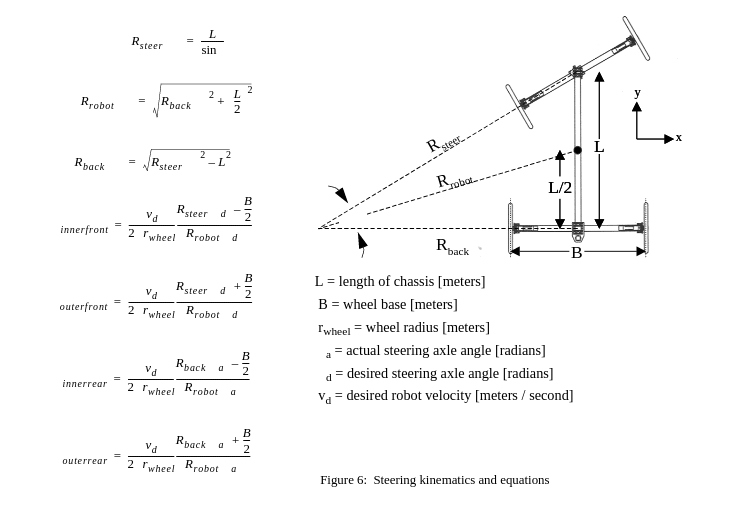
\includegraphics[width=\textwidth]{report_images/shamah.png}
\caption{(Shamah et. al. 2001)}
\end{figure}
Morgan Quigley, Brian Gerkey, Kevin Watts, Blaise Gassend authored a generic ROS joystick driver, which interfaces a joystick to ROS. This node is used for testing, and for teleoperation (Bohren, 2013).

\section{Materials and Components}
The materials, components and tools required to assemble the robot include:
\begin{itemize}
  \item 3D printed robot chassis
  \item 9 dynamixel AX-12 actuators with various length cables
  \item Screws of suitable length
  \item Raspberry Pi (model B or above) + wifi dongle
  \item USB2Dynamixel adapter
  \item 12V power source for the dynamixels
  \item 5V power source for the Pi
  \item \textit{Optional: soldering kit and heatshrink to properly splice a cable}
\end{itemize}
\subsection{Robot Chassis}
The Mantis chassis was printed with a Makerbot using PLA plastic. The printer was not particularly well calibrated and so the parts were all slightly too large. As a result, the assembly process was difficult but the overall result was acceptable.
\begin{figure}[H]
\centering
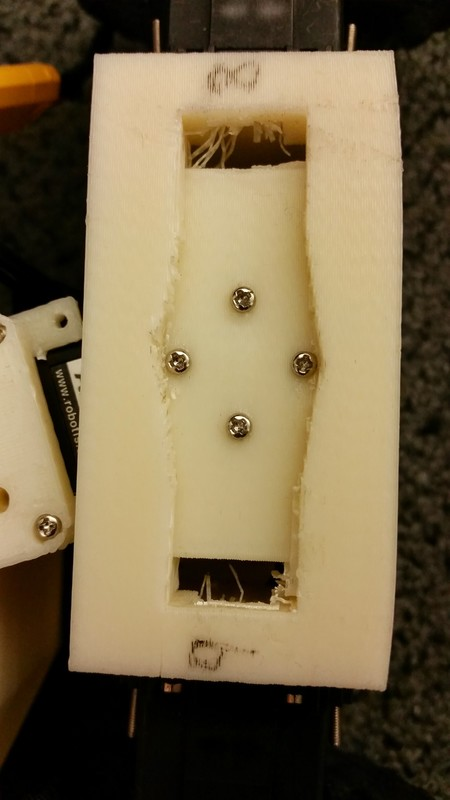
\includegraphics[width=200pt]{report_images/plastic_imperfection.jpg}
\caption{Very obvious imperfections, other parts are also less noticably wonky.}
\end{figure}
The main alternative to PLA plastic is ABS plastic. PLA plastic has a much lower melting point, which means that it may be subject to deformation if the dynamixel motors get too hot (the motors can heat up to 70 degrees celcius before shutting off). ABS plastic is stronger and generally favoured for more practical mechanical applications, but requires more complex printers with a heated bed. Both materials should be fine for use with Mantis (Chilson, 2013).
\\
\\
The wheels were also fully 3D printed, and one large issue is that they have very little grip on smooth surfaces such as wood. A possible solution is to coat the wheels in liquid/spray-on rubber. One such product is PlastiDip (PlastiDip, 2013).

\subsection{Dynamixel Motors}
\begin{figure}[H]
\centering
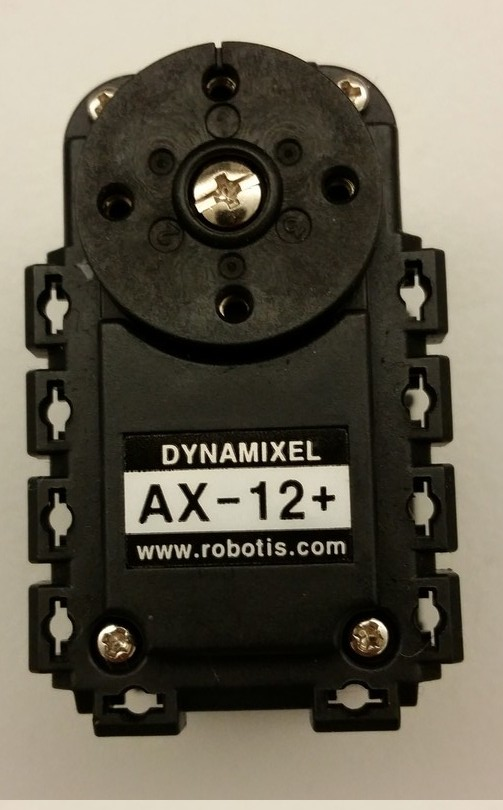
\includegraphics[width=80pt]{report_images/dynamixel.jpg}
\caption{A dynamixel AX-12+ which is newer than the AX-12 but older than the AX-12A}
\end{figure}
Mantis uses nine Dynamixel AX-12 motors. The dynamixel motors are fairly advanced compared to most motors and very good for a few reasons:
\begin{itemize}
  \item They are easily powered by 12V DC.
  \item They are able to function as both highly precise joints as well as wheels in wheel mode.
  \item They are chained together and all 9 motors are easily controlled from the Raspberry Pi
  \item There are existing libraries to interface with the dynamixels.
\end{itemize}
However, they are fairly expensive and make up the bulk of the cost of the OARKit. The dynamixel AX-12A currently sell for \$44.90 each (TrossenRobotics, 2014).
\\
\\
However there do not seem to be many alternatives - the AX-12 is already outstanding for its price point.

\subsection{The Brain}
A Raspberry Pi was used to control the 9 Dynamixel motors, as it is powerful enough for simple applications, has a fairly small physical footprint and has USB ports to connect to the USB2Dynamixel.
\begin{figure}[H]
\centering
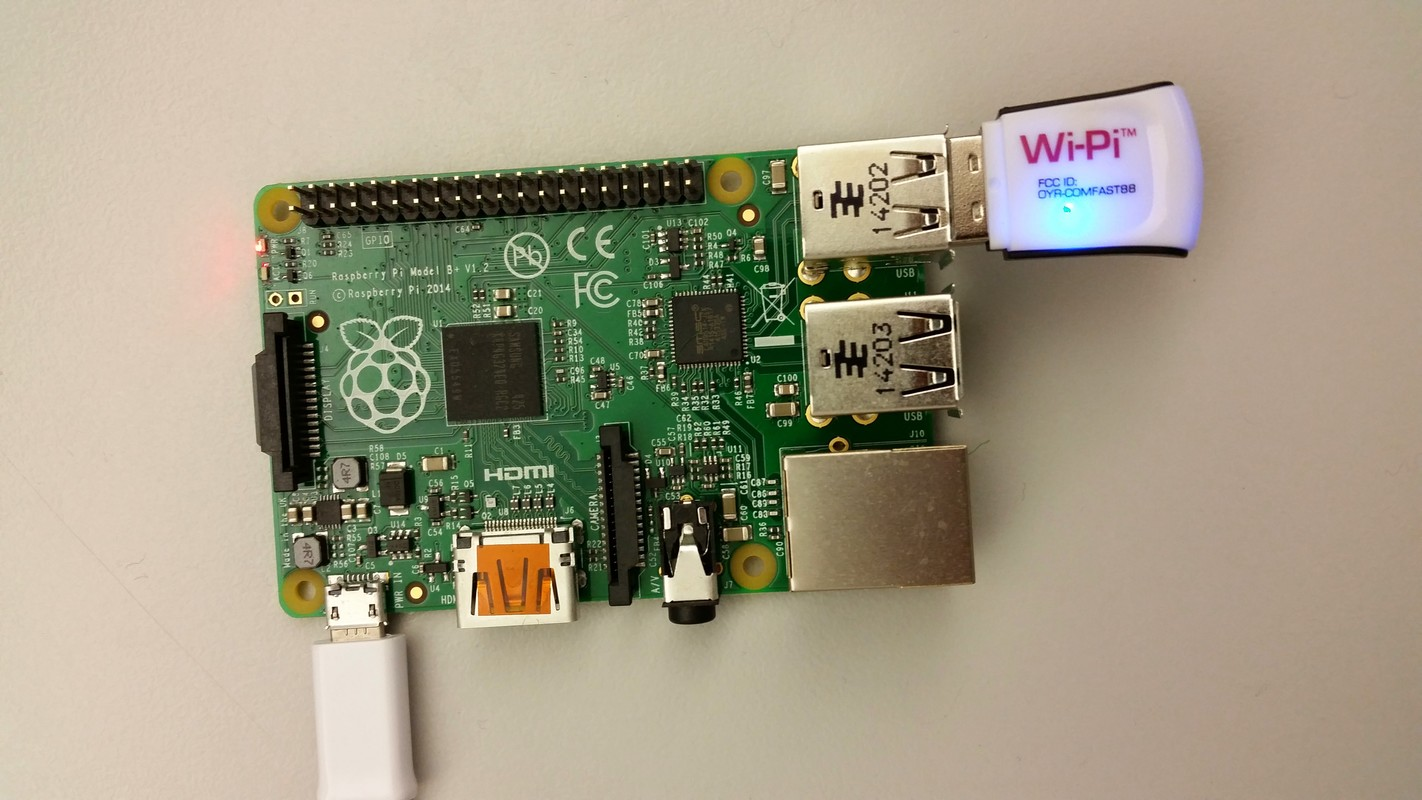
\includegraphics[width=200pt]{report_images/pi.jpg}
\caption{Raspberry Pi model B+, pictured with wifi dongle.}
\end{figure}
A model B or above is required because at least 2 USB ports are needed for the wifi dongle and the USB2Dynamixel.

\subsection{Power Sources}
The dynamixel motors accept 9-12V with a recommended voltage of 11.1V (Robotis, 2010).
\\
\\
The motors were supplied with a 12V power source via 8 AA batteries. A better alternative would be a 11 or 12V lithium-ion rechargable battery pack - this would be lighter, last longer and cheaper in the long run.
\begin{figure}[H]
\centering
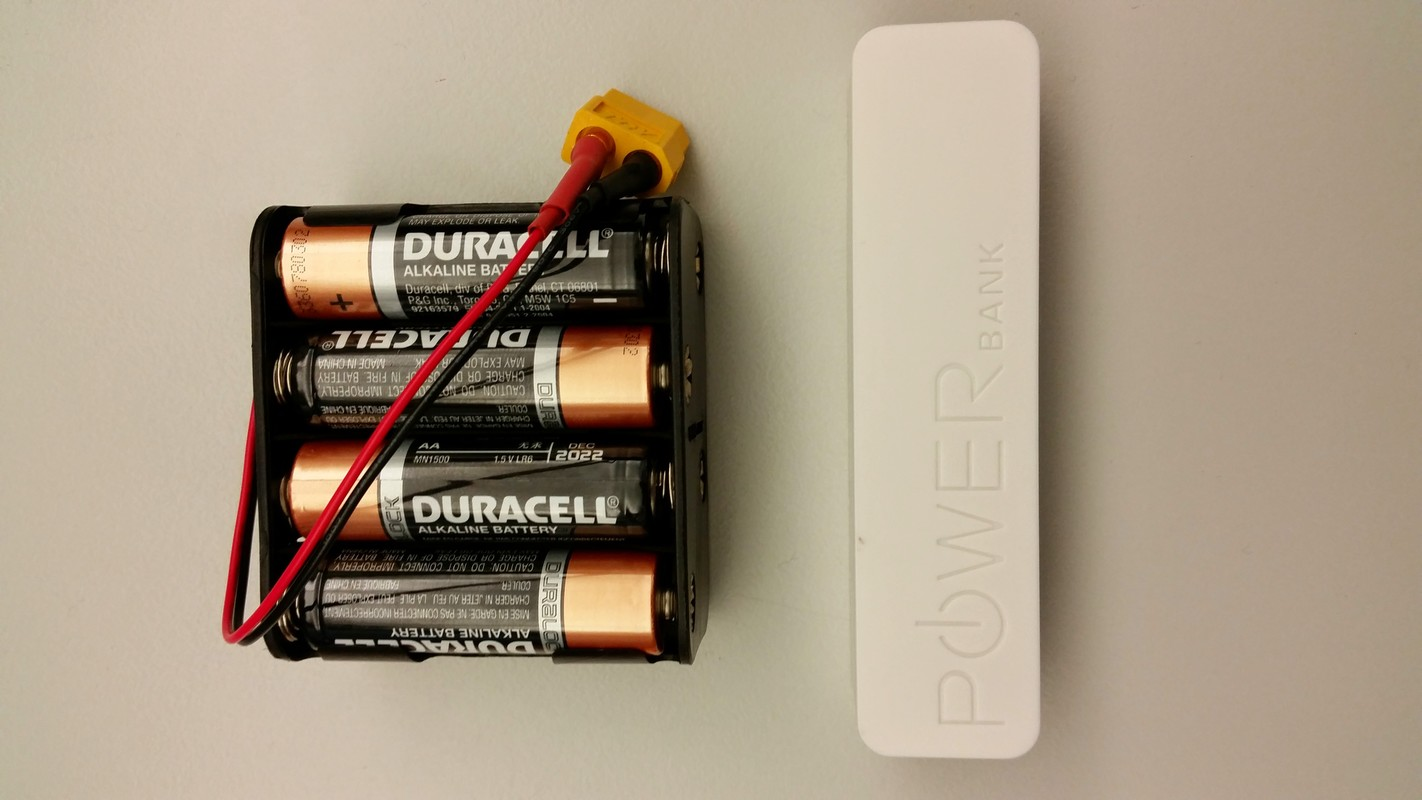
\includegraphics[width=200pt]{report_images/power_sources.jpg}
\caption{On the left, 12V power source from 8 AA batteries. On the right, a 5V rechargeable battery pack.}
\end{figure}
\begin{figure}[H]
\centering
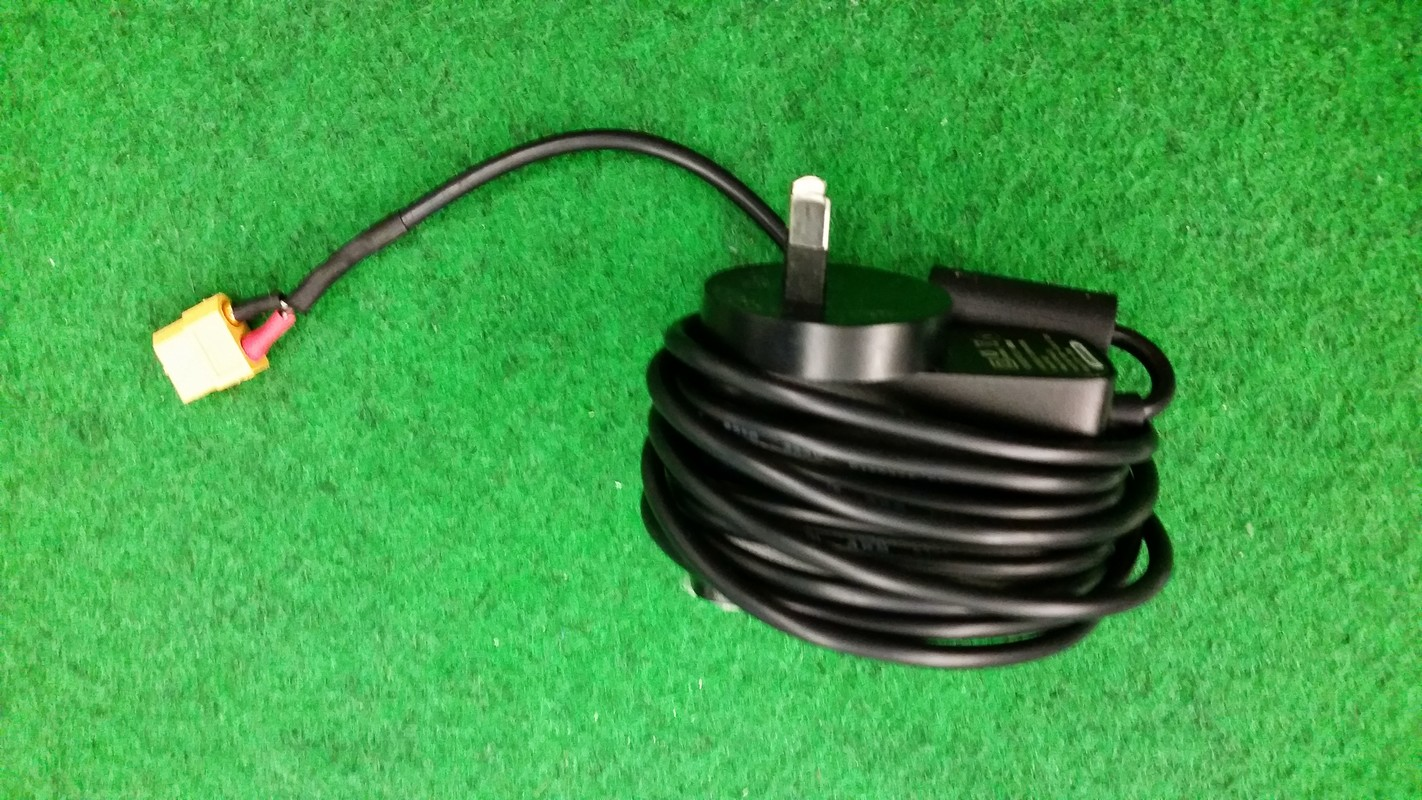
\includegraphics[width=200pt]{report_images/wall_power.jpg}
\caption{An optional 12V adapter that can be plugged into a wall socket for testing the mantis robot without having to go through too many batteries.}
\end{figure}
The Raspberry Pi requires a steady 5V power source via a mini-USB connector. An external battery pack for phones was used as a simple, rechargable power source, however ideally a more compact power source would be used, as the Mantis have very little onboard space.

\section{Assembly Process}
The assembly process consisted of attaching the printed plastic parts to the motors via screws. The Dynamixel Robot Actuator Kit provides nine different lengths of screws, from S1 (the shortest screw) to S9 (the longest screw), as well as nuts to help stabilise the attachment.
\begin{figure}[H]
\centering
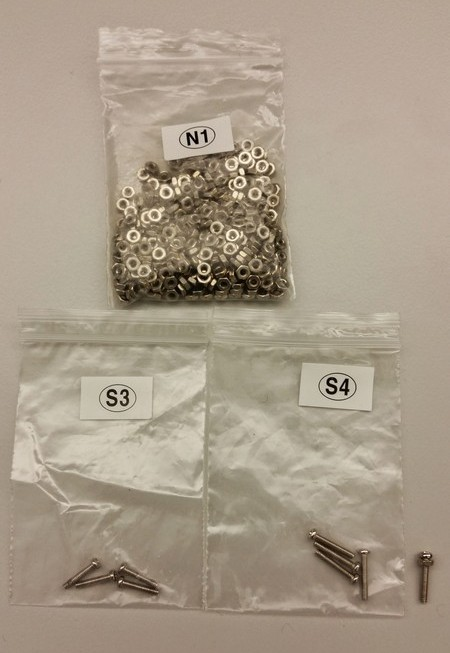
\includegraphics[width=80pt]{report_images/screws.jpg}
\caption{The most common screws that were used - S3 and S4. In the lower right hand corner is an S4 with a nut attached to shorten it.}
\end{figure}
The assembly was made difficult and inconsistent due to the low quality of the printed plastic - the surface was uneven and as the printer was not calibrated well the pieces were of an irregular size. As a result, the screws used were a mix of S2, S3, and S4 screws with nuts added in where more grip was required. It is difficult to define an effective specification for screw lengths for assembly without higher quality materials.
\begin{figure}[H]
\centering
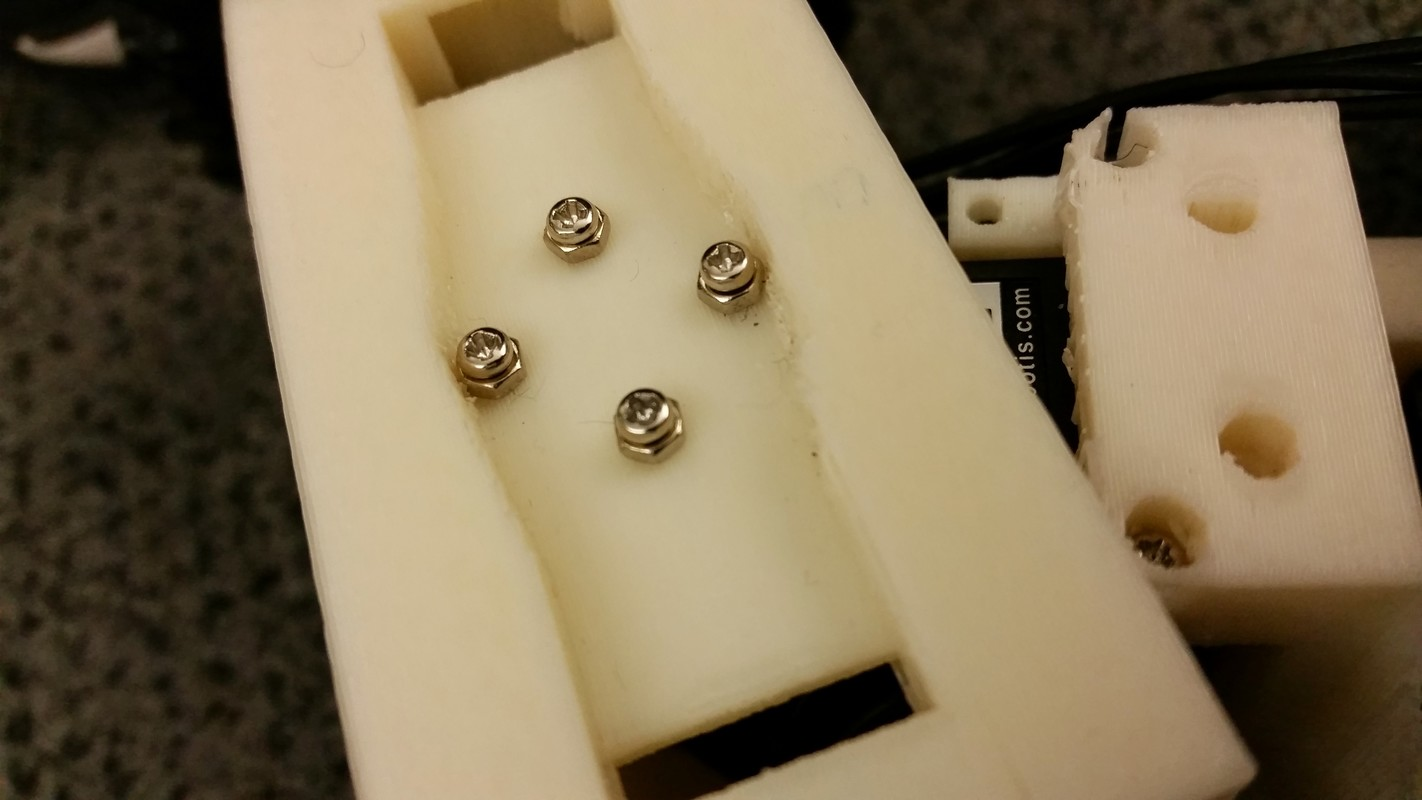
\includegraphics[width=200pt]{report_images/screw_nut.jpg}
\caption{An example of an S4 screw used in conjuction with a nut to provide a more suitable screw length.}
\end{figure} 
During assembly, there are certain screws that are very difficult to access. A very small phillips head screwdriver is recommended.
\begin{figure}[H]
\centering
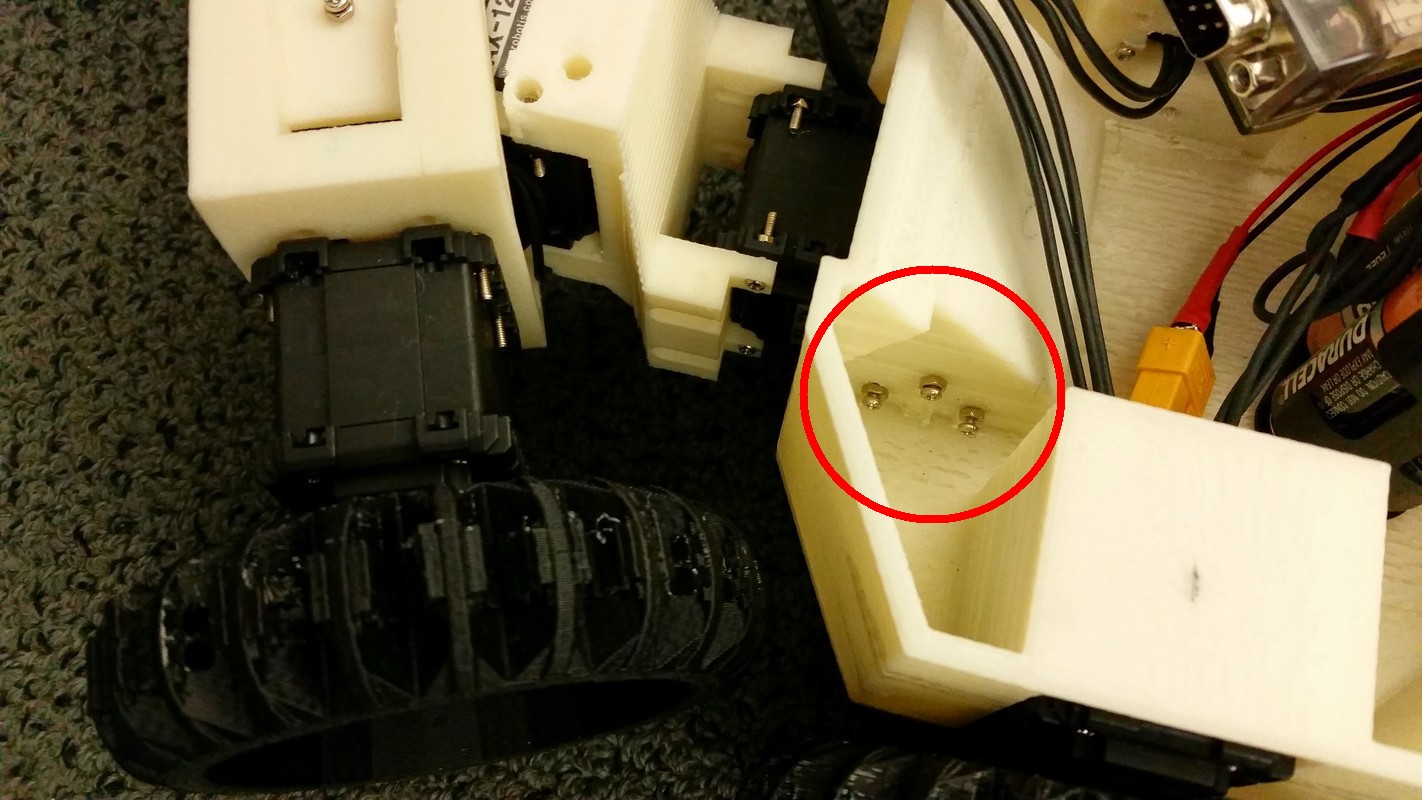
\includegraphics[width=200pt]{report_images/difficult_screw.jpg}
\caption{One of the more difficult set of screws to attach. A very short screwdriver and lots of patience is recommended.}
\end{figure}
There is a certain order of operations to follow: the cables which connect the dynamixels together must be plugged in before attaching the dynamixels to the chassis in many cases - it becomes very difficult after all the pieces are secured. This means that the order of the dynamixels must be determined ahead of time. Note that the actual ordering does not matter, as long as all the motors are connected on one network.
\begin{figure}[H]
\centering
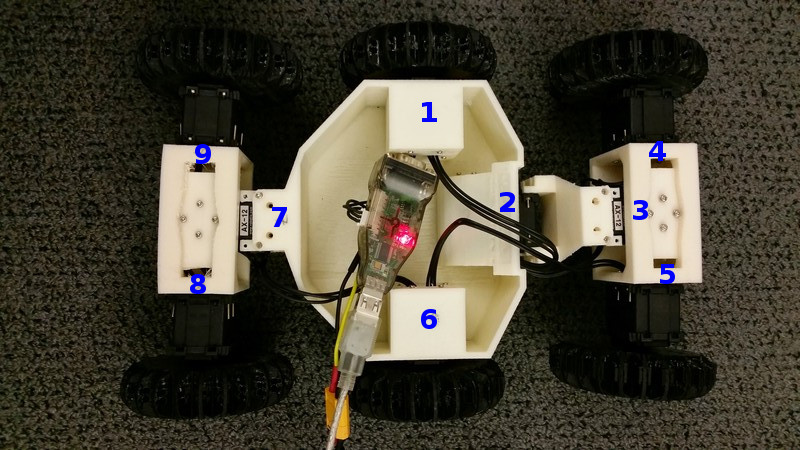
\includegraphics[width=200pt]{report_images/top_down.jpg}
\caption{The assembled mantis robot, with each dynamixel motor labeled in the order in which they were chained together. The USB2Dynamixel attaches to the motor labeled 1.}
\end{figure}
In order to power the dynamixel motors while using the USB2Dynamixel, the 12V power source must be spliced with the cable coming out of the data pin from the USB2Dynamixel in order to provide power and data.
\begin{figure}[H]
\centering
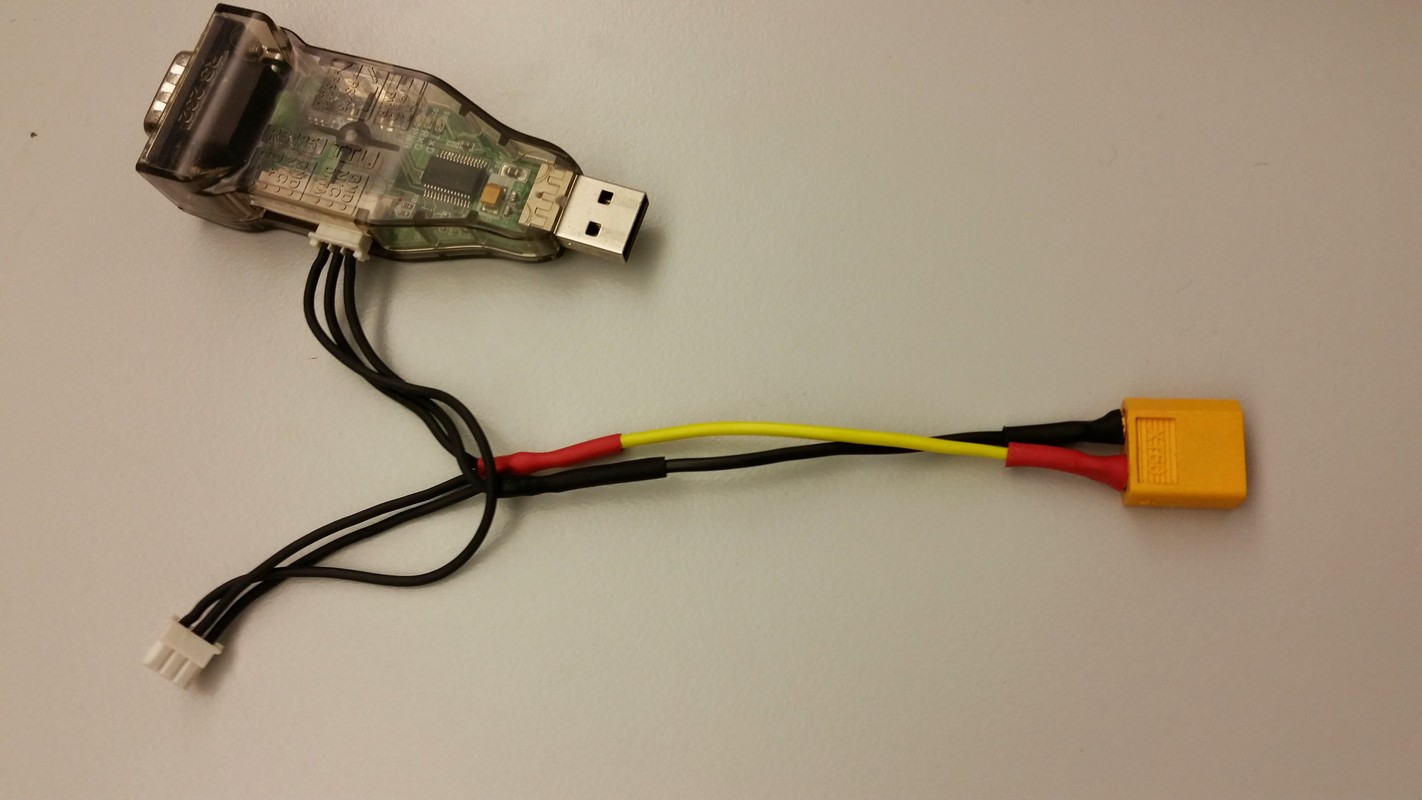
\includegraphics[width=200pt]{report_images/splice.jpg}
\caption{The three wires from left to right (as plugged into the USB2Dynamixel) carry data, 12V and ground respectively. Pictured is a sample spliced cable which connects the 12V power source and USB2Dynamixel to the dynamixel motors.}
\end{figure}

\section{Locomotion}
The OARKit robot has a fairly rare design in which six wheels can turn relative to each other via two rotating joints, each with a range of about $\pm20$ degrees.
\begin{figure}[ht]
    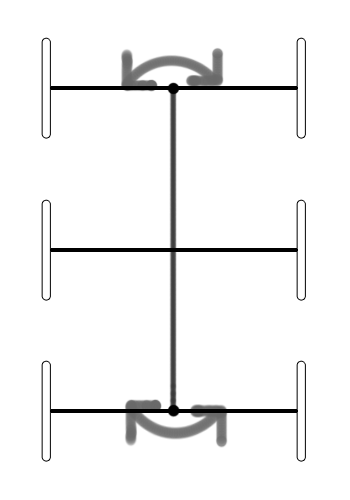
\includegraphics[height = 200pt]{report_images/diagram1.png}
    \caption{(A diagram of the articulated steering system of the OARKit robot.)}
    \label{fig:diagram1}
\end{figure}
There have been similar studies into wheel velocities for similar vehicles, such as Shamah et al. (2001)'s calculations diagrammed above, but the OARKit robot is unique in that it has mobile joints rather than rotating axles, and it also has six wheels for better locomotion.
\\
\\
We use similar calculations to Shamah et al., by definining a common intersection point for lines passing through all the axles, and using the distance between the wheel and the common intersection point to scale the relative velocity of the wheel.
\\
\begin{figure}[ht]
    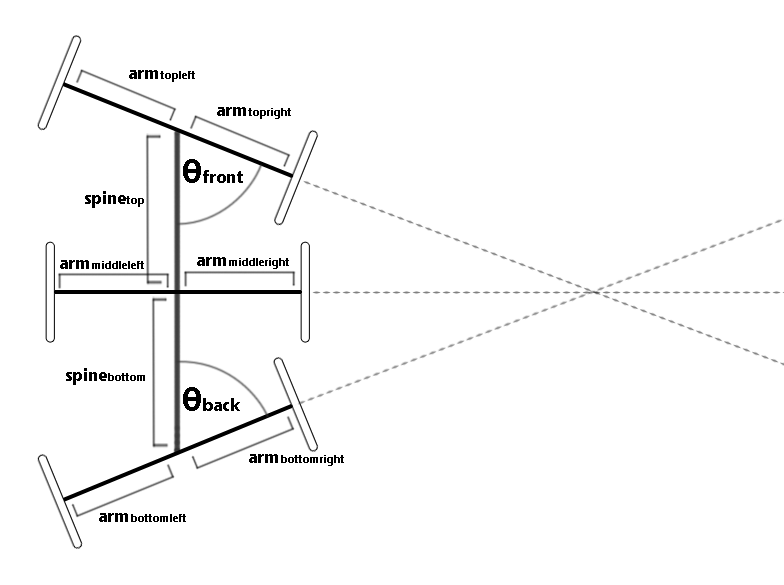
\includegraphics[height = 200pt]{report_images/diagram2.png}
    \caption{(The measurements we used in our calculations of wheel velocities)}
    \label{fig:diagram2}
\end{figure}
\\
Since we have six wheels and not four, there are six different axles. Thus we must make sure that the back axle is angled such that the line extended inwards would intersect with the intersection of the front two axle lines.
\\
\\
For $\theta_{front} > \frac{\pi}{2}$:
\[ \theta_{back} = tan^{-1}(tan(\theta_{front}) \times \frac{spine_{top}}{spine_{bottom}}) \]
\\
\\
For $\theta_{front} > \frac{\pi}{2}$:
\[ \theta_{back} = \pi - tan^{-1}(tan(\pi - \theta_{front}) \times \frac{spine_{top}}{spine_{bottom}}) \]
\\
\\
With the angle values of the top and bottom, we can thus define the relative velocities of all the wheels as the distances from the center point:
\\
\[ \omega_{topleft} \propto \frac{1}{sin(a)} + \frac{arm_{topleft}}{spine_{top} * tan(\theta_{top})} \]
\[ \omega_{topright} \propto \frac{1}{sin(1)} - \frac{arm_{topright}}{spine_{top} * tan(\theta_{top})} \]
\[ \omega_{middleleft} \propto 1 + \frac{arm_{midleft}}{spine_{top} * tan(\theta_{top})} \]
\[ \omega_{middleleft} \propto 1 - \frac{arm_{midright}}{spine_{top} * tan(\theta_{top})} \]
\[ \omega_{bottomleft} \propto \frac{spine_{bottom}}{spine_{top} * tan(\theta_{top}) * cos(\theta{bottom})} + \frac{arm_{bottomleft}}{spine_{top} * tan(\theta_{top})} \]
\[ \omega_{bottomleft} \propto \frac{spine_{bottom}}{spine_{top} * tan(\theta_{top}) * cos(\theta{bottom})} - \frac{arm_{bottomright}}{spine_{top} * tan(\theta_{top})} \]
\\
\\
We use this kind of articulated steering as the baseline velocity for all the wheels when the robot is at a certain inclination. Ideally this would cause all wheels to travel exactly at the correct tangential velocity.
\\
In our mantis library, we define the velocity of the vehicle $v$ as the tangential velocity of the center point of the middle axle (which is $spine_{top} * tan(\theta_{top})$ distance from the central intersection). We can multiply any of the above formulae by $v$ to obtain a velocity relative to the velocity of the center of the vehicle:
\\
\[ \omega_{topleft} = v * (\frac{1}{sin(a)} + \frac{arm_{topleft}}{spine_{top} * tan(\theta_{top})}) \]
\[ \omega_{topright} = v * (\frac{1}{sin(1)} - \frac{arm_{topright}}{spine_{top} * tan(\theta_{top})}) \]
\[ \omega_{middleleft} = v * (1 + \frac{arm_{midleft}}{spine_{top} * tan(\theta_{top})}) \]
\[ \omega_{middleleft} = v * (1 - \frac{arm_{midright}}{spine_{top} * tan(\theta_{top})}) \]
\[ \omega_{bottomleft} = v * (\frac{spine_{bottom}}{spine_{top} * tan(\theta_{top}) * cos(\theta{bottom})} + \frac{arm_{bottomleft}}{spine_{top} * tan(\theta_{top})}) \]
\[ \omega_{bottomleft} = v * (\frac{spine_{bottom}}{spine_{top} * tan(\theta_{top}) * cos(\theta{bottom})} - \frac{arm_{bottomright}}{spine_{top} * tan(\theta_{top})}) \]
\\
This method of locomotion is quite efficient - the wheels are all synchronised fairly well, and there is little drag of the tyres on the ground. However, one can also add a skid steering velocity onto the wheels on each side, sacrificing efficiency to be able to perform a tighter turn.
\\
\\
We implement this additively - there is a skid steering command available that will add a certain velocity to the wheels on each side of the robot, aiding turns greatly. For example, if a velocity of $2pi$ $m/s$ was added to one side, and a velocity of $-2pi$ $m/s$ was added to the other side, the vehicle would theoretically rotate at approximately $1 / radius$ revolutions per second along its current course, something not achievable with articulated steering. However, as mentioned before, since this is being performed on six wheels, there is a fair amount of drag between the wheels and the ground. This can be reduced by lifting up the front portion of the robot, so only four wheels are in contact with the ground.

\subsection{Results}
During testing, it was found that both methods of steering the Mantis were effective on wood and carpet surfaces. The six-wheeled skid steering had some issues on the carpet because the wheels gripped the surface too hard, but if the front portion of the robot was lifted up, there were no resulting problems. Additionally, the skid steering was unreliable and caused the robot to rotate differing angular distances on different surfaces.
\\
\\
However, the robot did also have the problem of not having enough grip. The wheels were constructed from PLA filament and had no coating, which means they had very little friction with the wooden surface and had some trouble performing maneuvers on sloped wooden surfaces, as it would slip down.
\\
\\
It was also noted that it was quite possible to reliably execute tight turns on multiple surfaces by using common vehicle maneuvers, such as three-point turns, in conjunction with articulated steering.

\subsection{Interface}
Several interface functions are provided in mantis.py that allow control of the robot with the designated steering system:
\begin{itemize}
    \item move(int -1023 to 1023): Move the robot at a given velocity (positive or negative). Path and direction is determined by current articulation.
    \item skid(int -1023 to 1023): Add a skid steering velocity to the current movement.
    \item turn\_to(int -1 to 1): Set the articulation to a given value between -1 (minimum articulation) and 1 (maximum articulation)
    \item lift\_to(int -1 to 1): Set the lift of the front segment to a given value between -1 and 1.
    \item turn(int -1023 to 1023): A convenience function that sets the robot to change its articulation at a certain speed until it reaches the maximum or minimum articulation.
    \item lift(int -1023 to 1023): Same as above, except with the lifting joint.
\end{itemize}

Multiple constants are defined which refer to all the dimensions and maximum and minimum turning points for the servomotors. These can be found in pyoarkit/config.py, and calibrated for individual robots. The default measurements are as follows:
\lstset{language=Python}
\begin{lstlisting}
# angles for top axle
CENTER_VALUE_TOP = 512.0 - 10.0  # 90 degrees
CENTER_ANGLE_TOP = radians(90.0)
MIN_VALUE_TOP = 512.0 - 110.0  # 65 degrees
MIN_ANGLE_TOP = radians(65.0)
MAX_VALUE_TOP = 512.0 + 100.0  # 115 degrees
MAX_ANGLE_TOP = radians(115.0)

# angles for bottom axle
CENTER_VALUE_BOTTOM = 512.0 + 10.0  # 90 degrees
CENTER_ANGLE_BOTTOM = radians(90.0)
MIN_VALUE_BOTTOM = 512.0 - 60.0  # 110 degrees
MIN_ANGLE_BOTTOM = radians(110.0)  # note min value gives a corresponding larger angle
MAX_VALUE_BOTTOM = 512.0 + 90.0  # 70 degrees
MAX_ANGLE_BOTTOM = radians(70.0)

# lengths of arms (mm)
ARM_TOP_LEFT = 91.0
ARM_TOP_RIGHT = 91.0
ARM_MID_LEFT = 95.0
ARM_MID_RIGHT = 95.0
ARM_BOTTOM_LEFT = 91.0
ARM_BOTTOM_RIGHT = 91.0

# lengths of spine (mm)
SPINE_TOP = 130.0
SPINE_BOTTOM = 120.0

# max velocity of any given wheel
MAX_WHEEL_VELOCITY = 1023.0

# limits for lift
MIN_LIFT_VALUE = 412
CENTER_LIFT_VALUE = 512
\end{lstlisting}

\section{Networking and Interface}
It is crucial for the robot to be able to communicate over the network in some form, so that it can operate without being tethered to cables. The onboard Raspberry Pi and dynamixel motors are equipped with portable power sources, and a wifi dongle allows the Pi to communicate over a network over wifi.

\subsection{A Sample Interface}
A sample interface has been designed to use the high level API functions provided by our pyOARKit library. Contained in interface.py, it can be run from the terminal and accepts input from the keyboard.
\\
\\
The interface is very simple and involves text-based commands of the form <command><value> where <command> is a single letter and <value> is typically an integer or a float.
\\
\\
\begin{tabular}{ | l | l | p{5cm} | }
\hline
\textbf{Syntax} & \textbf{Value Range} & \textbf{Description} \\ \hline
v<velocity> & Integer from -1023 to 1023 & Sets the velocity - moves the robot forwards and backwards. \\ \hline
s<velocity> & Integer from -1023 to 1023 & Skid steering - a positive value moves the right wheels forward and the rear wheels backwards. Can be used in conjunction with velocity setting. \\ \hline
t<velocity> & Integer from -1023 to 1023 & Turn at the given velocity - a positive value turns left. \\ \hline
l<velocity> & Integer from -1023 to 1023 & Lift the front segment up at the given velocity - a positive value lifts upwards \\ \hline
T<angle> & Float from -1 to 1 & Turn to the given normalised angle at an arbitrary speed of 50. 1 is the extreme left and -1 is the extreme right while 0 is the centre position. \\ \hline
L<angle> & Float from -1 to 1 & Lift to the given normalised angle at an arbitrary speed of 50. 1 is the maximum height and -1 is the minimum height while 0 is the centre position - flat. \\ \hline
\end{tabular}

\subsection{ROS Integration}
It was decided that the Mantis should be integrated with ROS in order to leverage the existing ecosystem of software and tools. Initially, the intention was to install ROS on the onboard Raspberry Pi but this proved to be complicated since ROS only officially compliant with Ubuntu. Furthermore, running ROS as well as controlling the nine dynamixel motors on the Pi would be difficult. The Pi (Model B+) only boasts 512mb of RAM and a 700MHz CPU, and it is unnecessary to increase cost with a more powerful microcomputer, when the processing could be delegated.
\\
\\
Instead, a small UDP server was run on the Pi and the ROS node was run on a desktop/laptop.

\subsubsection{server.py}
This is a small UDP server run on the Raspberry Pi and uses the sample interface.py. It accepts UDP messages which contain commands in the same format as the sample interface. From the Pi:
\begin{lstlisting}[language=bash]
  $ python server.py 9999 # Run the server on port 9999
\end{lstlisting}
\subsubsection{ROS Node}
This sample ROS node runs on a desktop or laptop and sends UDP messages to the server on the Pi based on input from a joystick. A logitech controller was used when demonstrating, but the code should be able to be easily adapted for other joysticks or similar teleop nodes. Ensure that the joystick is plugged in, and then:
\begin{lstlisting}[language=bash]
  $ sudo apt-get install ros-indigo-joystick-drivers # Make sure you have the joystick drivers
  $ roslaunch logitech.launch
  $ cd workspace
  $ catkin_make
  $ rosrun mantis move.py <ip_of_raspberry_pi> 9999 # Connect to the Pi on port 9999
\end{lstlisting}

\subsubsection{Logitech Joystick}
The Logitech joystick should now be able to control the Mantis. The control scheme is as follows:
\\
\\
\begin{tabular}{ | l | p{7cm} | }
\hline
\textbf{Control} & \textbf{Description} \\ \hline
Left joystick up and down & Moves the robot forwards and backwards. \\ \hline
Left joystick left and right & Performs skid steering on the robot. \\ \hline
Right joystick up and down & Raise and lower the front segment of the robot. \\ \hline
Right joystick left and right & Turn the robot left and right. \\ \hline
Hold Start button & Return the robot to the neutral position - turn to face forwards and raise/lower the front segment to be parallel to the ground. \\ \hline
\end{tabular}

\subsection{Design Decisions and Potential Issues}
The main decision to make was to decide on the protocol used to send messages from the ROS node to the server on the Pi. UDP was chosen over TCP or any other protocols because being able to control the robot in real time was a priority. There were potentially a lot of messages being sent very quickly when moving the joystick and using TCP could have caused some unwanted delay.
\\
\\
Dropped packets are not a large issue (UDP does not guarantee delivery) because the interface and library are mostly stateless. That is, subsequent commands are mutually exclusive and do not affect one another. At worst, it would just require inputting a particular command again. However, an issue was observed, where actions on the joystick sometimes would not register. The issue was pinpointed to a few potential sources:
\begin{enumerate}
  \item Dropping packets over the network
  \item Congestion in the dynamixel network causing commands sent to the dynamixels to not take effect
  \item Incorrect report from the joystick itself
\end{enumerate}
The server and client was changed to use TCP instead of UDP, but the issue persisted. It also seems unlikely that there would be a hardware issue with the joystick or the joystick drivers but we were unable to verify this.
\\
\\
A possible solution could be to try lowering the rate at which commands are sent to the dynamixels (currently every 0.2 seconds). However, this would likely introduce noticeable input delay.
\\
\\
During the demonstration, movement was heavily delayed. A possible issue is a congested network during the day, since we operated on the unviersity wireless network available to everyone. An ad-hoc network directly connecting the Pi to a laptop could have been a solution, but we were unable to test this.
\\
\\
During the demonstration very heavy delays were experienced, and commands on the joystick would frequently fail to register, especially lifting the front segment. However, after cleaning up and restructuring the code, subsequent testing found the system to be very responsive and unregistered commands were fairly rare. At this point it is unclear whether it was an issue with the code or a more congested wifi network at the time of demonstration.

\section{Conclusion}
The aim of the project was to write a suite of software for the Open Academic Robot Kit which would provide locomotion, networking and compatibility with ROS. We created a library exposing a high level API for locomotion, and a networking model that was able to integrate with ROS and facilitate control of the robot with a Logitech controller.
\\
\\
The final result is a cheap, accessible 3D-printed robot able to be controlled wirelessly. Despite the poor performance during the demonstration, after fixing some issues and more testing the mantis robot does respond well to real-time input.

\subsection{Future Work}
While significant progress has been made, there is still plenty of additional work that could be done.
\\
\\
OARKit also contains an optional movable arm which holds a camera or sensor. Additional software could be written to move the arm appropriately and process the camera or sensor data. Perhaps a more powerful onboard controller would work better here to be able to do some of the image processing locally.
\\
\\
Currently the parts do not fit very well inside the main body of the robot chassis. The USB2Dynamixel, while convenient, is very bulky and is the main culprit of this problem. It can be removed if the Pi interfaces with the dynamixel motors directly via serial pins. //TODO cite people talking about how need additional gate/circuit.


\section{References}
Bigge, R. (2011). \textit{Robots to the rescue}. Available at\\
https://secure.globeadvisor.com/servlet/ArticleNews/story/gam/20110527\\
/ROBMAG\_JUNE2011\_P12\_14\_ (accessed 04/11/2014).\\
\\
Bohren, J. (2013). \textit{joy}. Available at http://wiki.ros.org/joy. (accessed 12/11/2014).\\
\\
Chilson, L. (2013). \textit{The difference between ABS and PLA for 3D printing}. Available at http://www.protoparadigm.com/news-updates/the-difference-between-abs-and-pla-for-3d-printing/. (accessed 12/11/2014).
Davids, A. (2002). Urban search and rescue robots: from tragedy to technology. \textit{Intelligent Systems, IEEE 17}(2). 81 - 83.\\
\\
Gindel, P. (2010). \textit{Arduino library for AX-12}. \\Available at http://www.pablogindel.com/2010/01/biblioteca-de-arduino-para-ax-12/. (accessed 09/11/14).\\
\\
Kang, J., Kim W., Lee, J., \& Yi, K. (2010). Design, implementation, and test of skid steering-based autonomous driving controller for a robotic vehicle with articulated suspension. \textit{Journal of Mechanical Science and Technology 24}(3). 793 - 800.\\
\\
Kobe University Library. (1999) \textit{Great Hanshin-Awaji Earthquake Disaster Materials Collection.} Available at: http://www.lib.kobe-u.ac.jp/eqb/e-gallery.html (accessed 04/11/2014).\\
\\
The Open Academic Robotic Kit. Available at www.oarkit.org (accessed 09/11/2014).\\
\\
PlastiDip. (2013). \textit{Plastic Dips and Coatings}. Available at https://www.plastidip.net.au/. (accessed 12/11/2014).\\
\\
Robotis. (2010). \textit{ROBOTIS e-Manual AX-12/ AX-12+/ AX-12A}. Available at http://support.robotis.com/en/product/dynamixel/ax\_series/dxl\_ax\_actuator.htm. (accessed 12/11/2014).\\
\\
Shamah, B.,  Wagner, M. D., Moorehead S., Teza, J., Wettergreen, D., \& Whittaker, W. (2001). \textit{Steering and Control of a Passively Articulated Robot}. The Field Robotics Center, Carnegie Mellon University.\\
\\
Sheh, R. (2014). \textit{Open Academic Robot Kit: The Six-Wheeled Wonder - a 6 Wheel Drive robot platform using Dynamixel AX-12A servos}. Available at: http://www.thingiverse.com/thing:327689 (accessed 04/11/2014).\\
\\
TrossenRobotics. (2014). \textit{Dynamixel AX-12A Robot Actuator}. Available at http://www.trossenrobotics.com/dynamixel-ax-12-robot-actuator.aspx. (accessed 12/11/14).

\end{document}
